%% \documentclass[handout,t]{beamer} % HANDOUT
%% \documentclass[handout,notes=show,t]{beamer} % NOTES
\documentclass[t]{beamer} % SLIDES

\usetheme{SIGIL}
\usepackage{beamer-tools-sigil}

%%
%%  INCLUDE: math.tex
%%  
%%  basic mathematical symbols and constructs (not specific to cooccurrences)
%%


%% \setN, \setN[0], \setZ, \setQ, \setR, \setC
%% abbreviations for common number spaces
\newcommand{\setN}[1][]{\mathbb{N}_{#1}} % allows \setN and \setN[0]
\newcommand{\setZ}{\mathbb{Z}}
\newcommand{\setQ}{\mathbb{Q}}
\newcommand{\setR}{\mathbb{R}}
\newcommand{\setC}{\mathbb{C}}

%% \set{el_1, el_2, ...};  \setdef{el}{condition};  \bigset{..}, \bigsetdef{..}{..}
%% extensional and intensional definition of sets, with "big" versions (like \bigl etc.)
\newcommand{\set}[1]{\left\{#1\right\}}
\newcommand{\setdef}[2]{\set{#1\,\left|\,#2\right.}}
\newcommand{\bigset}[1]{\bigl\{#1\bigr\}}
\newcommand{\bigsetdef}[2]{\bigset{#1\bigm|#2}}
\newcommand{\Bigset}[1]{\Bigl\{#1\Bigr\}}
\newcommand{\Bigsetdef}[2]{\Bigset{#1\Bigm|#2}}
\newcommand{\biggset}[1]{\biggl\{#1\biggr\}}
\newcommand{\biggsetdef}[2]{\biggset{#1\biggm|#2}}

%% \compl{X} = complement of set X
\newcommand{\compl}[1]{\mathcal{C} #1}

%% \eps == \epsilon, \si == \sigma, \sisi == \sigma^2, \ka == \kappa
\newcommand{\eps}{\epsilon}
\newcommand{\si}{\sigma}
\newcommand{\sisi}{\sigma^2}
\newcommand{\ka}{\kappa}

%% \abs{expr}, \bigabs{expr}, \norm{expr}, \bignorm{expr}
%% absolute value and norm of expression, with "big" versions
\newcommand{\abs}[1]{\left\lvert#1\right\rvert}
\newcommand{\bigabs}[1]{\bigl\lvert#1\bigr\rvert}
\newcommand{\norm}[1]{\left\lVert#1\right\rVert}
\newcommand{\bignorm}[1]{\bigl\lVert#1\bigr\rVert}

%% \constpi == constant PI (in bold font)
\newcommand{\constpi}{\boldsymbol{\pi}}

%% \dx == "dx";  \dx[z] == "dz";  \dpi == \dx[\pi];  
%% \dG == \dx[G], \dt == \dx[t]
\newcommand{\dx}[1][x]{\,d#1}
\newcommand{\dpi}{\dx[\pi]}
\newcommand{\dG}{\dx[G]}
\newcommand{\dt}{\dx[t]}

%% \Int{\frac{1}{2} x^2}_a^b
%% anti-derivative evaluated to compute definite integral
\newcommand{\Int}[1]{\left[#1\right]}

%% \limdownto{x}{0}
%% limit from above for x -> 0
\newcommand{\limdownto}[2]{\lim_{#1\,\downarrow\,#2}}

%% \iffdef == ":<=>";  \iffdefR == "<=>:"
\newcommand{\iffdef}{\;:\!\iff}
\newcommand{\iffdefR}{\iff\!:\;}

%% \logten(x) 
%% base 10 logarithm, which is always used in the UCS system
\newcommand{\logten}{\log_{10}}

%% \e+3, \e-6, \e-{12}, 5.5\x\e-3
%% engineering-style notation (orders of magnitude) for floating-point numbers
\newcommand{\e}[2]{10^{\ifthenelse{\equal{#1}{+}}{}{#1}#2}}
\newcommand{\x}{\cdot}

%% \Landau{ n^2 }, \bigLandau{ N^2 }
%% Landau symbol ("big oh notation")
\newcommand{\Landau}[1]{\mathcal{O}\left({#1}\right)}
\newcommand{\bigLandau}[1]{\mathcal{O}\bigl({#1}\bigr)}


%%% Local Variables: 
%%% mode: latex
%%% TeX-master: t
%%% End: 
  % basic mathematical notation
%%
%%  INCLUDE: stat.tex
%%  
%%  symbols and notation for probability theory and statistics
%%


%% \p{X=k};  \pC{X=k}{Y=l};  \pscale{\frac{Z}{S^2}}
%% probability P(X=k), conditional probability P(X=k|Y=l), and variants with scaled parentheses
\newcommand{\p}[1]{\mathop{\mathrm{Pr}}\bigl(#1\bigr)}
\newcommand{\pscale}[1]{\mathop{\mathrm{Pr}}\left(#1\right)}
\newcommand{\pC}[2]{\p{#1\bigm|#2}} 
\newcommand{\pCscale}[2]{\pscale{#1\,\left|\,#2\right.}} 

%% \Exp{X};  \Var{X};  \Exp[0]{X};  \Var[0]{X};  \Expscale{X};  \Varscale{X}
%% expectation E[X] and variance V[X], expectation and variance under null hypothesis, 
%% and variants with scaled brackets
\newcommand{\Exp}[2][]{E_{#1}\bigl[#2\bigr]}
\newcommand{\Var}[2][]{\mathop{\mathrm{Var}}_{#1}\bigl[#2\bigr]}
\newcommand{\Expscale}[2][]{E_{#1}\left[#2\right]}
\newcommand{\Varscale}[2][]{\mathop{\mathrm{Var}}_{#1}\left[#2\right]}

%% \I{f_i = M};  \bigI{\sum_{i=1}^S f_i = N}
%% indicator variable (as in Baayen 2001), and variant with explicitly scaled brackets
\newcommand{\I}[1]{I_{\left[#1\right]}}
\newcommand{\bigI}[1]{I_{\bigl[#1\bigr]}}

%% \Hind;  \Hhom;  \Hnull{\kappa = x}
%% null hypothesis of independence and homogeneity; general null hypothesis identified by condition
\newcommand{\Hind}{H_0}
\newcommand{\Hhom}{H_{0,\, hom}}
\newcommand{\Hnull}[1]{H_{#1}}

%% \confint{\kappa};  \confint[0.99]{\kappa}
%% confidence interval for specified population characteristic (conf. level defaults to \alpha)
\newcommand{\confint}[2][\alpha]{I_{#2,\,#1}}

%% \df = 1
%% degrees of freedom
\newcommand{\df}{\mathit{df}}


%%% Local Variables: 
%%% mode: latex
%%% TeX-master: t
%%% End: 
  % notation for probability theory and statistics
%%
%% convenience macros for linear algebra (vectors and matrices)
%%

%% \Vector[i]{x} ... vector variable with optional _superscript_ index in parentheses
%% \Vector[']{x} ... special case: ' superscript not enclosed in parentheses
%% \vx, \vy, \vz ... abbreviations for common vector names
\newcommand{\Vector}[2][]{\mathbf{#2}\ifthenelse{\equal{#1}{}}{}{^{(#1)}}}
\newcommand{\vx}[1][]{\Vector[#1]{x}}
\newcommand{\vy}[1][]{\Vector[#1]{y}}
\newcommand{\vz}[1][]{\Vector[#1]{z}}
\newcommand{\vu}[1][]{\Vector[#1]{u}}
\newcommand{\vv}[1][]{\Vector[#1]{v}}
\newcommand{\vw}[1][]{\Vector[#1]{w}}
\newcommand{\vm}[1][]{\Vector[#1]{m}} 
\newcommand{\va}[1][]{\Vector[#1]{a}} % vectors of coefficients
\newcommand{\vb}[1][]{\Vector[#1]{b}} % for basis
\newcommand{\ve}[1][]{\Vector[#1]{e}} % for standard basis of R^n
\newcommand{\vn}[1][]{\Vector[#1]{n}} % normal vector
\newcommand{\vnull}[1][]{\Vector[#1]{0}} % neutral element

%% \Span{\vb[1],\ldots,\vb[k]} ... span of set of vectors
%% \Rank{...} ... rank of set of vectors or matrix
%% \Det{...}, \det A ... determinant of a set of vectors / a matrix A
%% \Image{f}, \Kernel{f} ... image and kernel of a linear map
\newcommand{\Span}[1]{\mathop{\text{sp}}\left(#1\right)}
\newcommand{\Rank}[1]{\mathop{\text{rank}}\left(#1\right)}
\newcommand{\Det}[1]{\mathop{\text{Det}}\left(#1\right)}
%% \det is already defined in the standard library
\newcommand{\Image}[1]{\mathop{\text{Im}}\left(#1\right)}
\newcommand{\Kernel}[1]{\mathop{\text{Ker}}\left(#1\right)}

%% \dist[2]{\vx}{\vy} ... distance between two vectors (p-metric)
\newcommand{\dist}[3][]{d_{#1}\left(#2, #3\right)}
\newcommand{\bigdist}[3][]{d_{#1}\bigl(#2, #3\bigr)}

%% \sprod{\vu}{\vv} ... scalar product
\newcommand{\sprod}[2]{\left\langle #1, #2 \right\rangle}
\newcommand{\bigsprod}[2]{\bigl\langle #1, #2 \bigr\rangle}


%%% Local Variables: 
%%% mode: latex
%%% TeX-master: ""
%%% End: 
% convenience macros for vectors and matrices

%%%
%%% local configuration adjustments
%%%

%%% You can change pre-defined colours here, override built-in macros from the
%%% style definition and standard library, as well as define macros needed by
%%% all local documents.

%%% e.g. adjust counterpoint (dark green) for data projectors where greens are
%%% far too bright, as well as green component of light colour and pure green
%%% (of course, it's a better solution to adjust the gamma settings of your monitor)
%%
%% \definecolor{counterpoint}{rgb}{.1, .3, 0}
%% \definecolor{light}{rgb}{.45, .3, .55}
%% \definecolor{puregreen}{rgb}{0, .35, 0}

%% ----- extra packages we need to load

\usepackage{tikz}
\usepackage{alltt}              % code examples with nicely formatted comments
\usepackage{rotating}


%% ----- author and copyright messages (so updates are automatically inserted into all files)
\newcommand{\sigilauthors}{%
  \author[SIGIL]{Designed by Stefan Evert\inst{1} and Marco Baroni\inst{2}}
  \institute[Evert \& Baroni]{
    \inst{1}Computational Corpus Linguistics Group\\
    Friedrich-Alexander-Universit�t Erlangen-N�rnberg, Germany
    \and
    \inst{2}Center for Mind/Brain Sciences (CIMeC)\\
    University of Trento, Italy
  }
}
\newcommand{\sigilcopyright}{%
  \date[sigil.r-forge.r-project.org]{%
    \primary{\footnotesize\url{http://SIGIL.r-forge.r-project.org/}}\\
    \light{\tiny Copyright \textcopyright\ 2007--2018 Evert \& Baroni}}
}

%% ----- automatically show TOC reminder at beginning of each subsection
\AtBeginSubsection[]
{
  \begin{frame}
    \frametitle{Outline}
    \tableofcontents[current,currentsubsection]
  \end{frame}
}

%% ----- some useful macros for the SIGIL course

\newenvironment{Rcode}[1][]{%
  \setbeamercolor{block title}{fg=counterpoint,bg=counterpoint!15!white}%
  \setbeamercolor{block body}{bg=counterpoint!5!white}\small%
  \begin{block}{#1}\begin{alltt}\ungap[1]}{%
      \ungap[1]\end{alltt}\end{block}} % \end{alltt} ... to deconfuse emacs

%% use \sbox{\Rbox} ... \usebox{\Rbox} to insert arbitray latex into Rcode environment
\newsavebox{\Rbox}

%% > plot(x,y)      \REM{this produces a scatterplot}
\newcommand{\REM}[2][\small]{\textsf{#1\color{primary}\# #2}}

%% nice colour for R output: \begin{Rout} .. \end{Rout}
\newenvironment{Rout}[1][\footnotesize]{%
  \begin{footnotesize}#1\color{secondary}\bfseries}{%
    \color{black}\mdseries\end{footnotesize}}

%% rotated column labels for table (to fit long text into narrow columns
\newcommand{\rotLabel}[2][60]{\begin{rotate}{#1}#2\end{rotate}}
 % local adjustments to configuration and macros

%%%%%%%%%%%%%%%%%%%%%%%%%%%%%%%%%%%%%%%%%%%%%%%%%%%%%%%%%%%%%%%%%%%%%%
%% Titlepage

\title[7.\ Multivariate Analysis]{Unit 7: Multivariate Analysis}
\subtitle{Statistics for Linguists with R -- A SIGIL Course}
\sigilauthors
\date[sigil.r-forge.r-project.org]{%
  \light{\tiny \sigilcopyright}}

\begin{document}

\frame{\titlepage}

%%%%%%%%%%%%%%%%%%%%%%%%%%%%%%%%%%%%%%%%%%%%%%%%%%%%%%%%%%%%%%%%%%%%%%

\section*{Outline}
\frame{ 
  \frametitle{Outline}
  \tableofcontents
}

%%%%%%%%%%%%%%%%%%%%%%%%%%%%%%%%%%%%%%%%%%%%%%%%%%%%%%%%%%%%%%%%%%%%%%
\section{Introduction}

%%%%%%%%%%%%%%%%%%%%%%%%%%%%%%%%%%%%%%%%%%
\subsection{Multivariate analysis}

\begin{frame}
  \frametitle{What is multivariate analysis?}

  \begin{itemize}
  \item Univariate statistics
    \begin{itemize}
    \item focus on a single variable of interest (at a time)
    \item estimate population parameters ($\pi$, $\mu$, $\sigma^2$, \ldots)
    \item comparison of two or more groups
    \end{itemize}
  \item<2-> Bivariate statistics
    \begin{itemize}
    \item focus on interdependencies of two variables
    \item correlation \& co-occurrence
    \end{itemize}
  \item<3-> Regression modelling
    \begin{itemize}
    \item predict single target variable (``dependent'')
    \item based on multiple other variables (``independent'')
    \end{itemize}
  \item<4-> Multivariate statistics
    \begin{itemize}
    \item combined effects of many variables
    \item correlations \& distribution patterns
    \item often ``unsupervised'': no target variable or comparison groups
    \end{itemize}
  \end{itemize}
\end{frame}

\begin{frame}
  \frametitle{Application examples}

  \begin{itemize}
  \item Register variation \citep{Biber:88,Biber:93}
  \item Translation studies\\ \citep{Evert:Neumann:16,DeSutter:Delaere:Plevoets:12}
  \item Stylometry: authorshop attribution \citep{Evert:etc:17}
  \item Dialectology \citep{Speelman:Grondelaers:Geeraerts:03}
  \item Historical linguistics \citep{Sagi:Kaufmann:Clark:09,Perek:18}
  \item Identification of confounding variables \citep{Tummers:Speelman:Geeraerts:14}
  \item Linguistic productivity \citep{Jenset:McGillivray:12}
  \item Correspondence analysis \citep{Greenacre:07}
  \item Distributional semantics (see \href{http://wordspace.collocations.de/doku.php/course:esslli2018:start}{\secondary{ESSLLI course}})
  \end{itemize}
\end{frame}

%%%%%%%%%%%%%%%%%%%%%%%%%%%%%%%%%%%%%%%%%%
\subsection{Setting up}

\begin{frame}
  \frametitle{R packages}
  % \framesubtitle{}

  Required R packages:
  \begin{itemize}
  \item \code{corpora} ($\geq$ 0.5)
  \item \code{wordspace} ($\geq$ 0.2)
  \end{itemize}

  Recommended packages:
  \begin{itemize}
  \item \code{ggplot2}, \code{reshape2} \ldots\ for plotting feature weights
  \item \code{rgl} \ldots\ for interactive 3-d visualization
  \item \code{Hotelling}, \code{ellipse} \ldots\ for significance testing
  \item \code{e1071} \ldots\ for machine learning (SVM)
  \item \code{Rtsne} \ldots\ for low-dimensional maps
  \item \code{ca} \ldots\ for correspondence analysis
  % \item \code{} \ldots\ for
  \item[]
  \end{itemize}

  \hand{} install with package manager in RStudio or R GUI
\end{frame}

\begin{frame}[fragile]
  \frametitle{Code \& data sets}
  % \framesubtitle{}

  Download additional code \& data sets from SIGIL homepage:
  \begin{itemize}
  \item \href{http://www.stefan-evert.de/SIGIL/sigil_R/materials/multivar_utils.R}{\code{gma\_utils.R}}
  \item \href{http://www.stefan-evert.de/SIGIL/sigil_R/data/unit7_data.rda}{\code{unit7\_data.rda}}
  \item[]
  \end{itemize}

  \hand{} put all files in RStudio project directory (or working directory)

  \gap[1]
\begin{Rcode}
> library(corpora)           \REM{basic utilities and some data sets}
> library(wordspace)         \REM{for large and sparse matrices}

> source("gma_utils.R")      \REM{additional functions}

> load("unit7_data.rda", verbose=TRUE) \REM{further data sets}
\end{Rcode}
\end{frame}

\begin{frame}
  \frametitle{Overview of data sets}

  \begin{itemize}
  \item 65 Biber features for British National Corpus
    \begin{itemize}
    \item \code{BNCbiber} = $4048\times 65$ feature matrix
    \item \code{BNCmeta} = complete metadata table
    \item extensive documentation with \code{?BNCbiber}, \code{?BNCmeta}
    \item[]
    \end{itemize}
  \item 67 Biber features for Brown Family corpora
    \begin{itemize}
    \item \code{BrownBiber\_Matrix} = $3500 x 67$ feature matrix
    \item \code{BrownBiber\_Meta} = metadata table
    \item features are Biber-scaled z-scores obtained with MAT v1.3\\
      {\footnotesize\secondary{\url{http://sites.google.com/site/multidimensionaltagger/}}}
    \item see tagger manual for feature definitions
    \end{itemize}
  \end{itemize}
\end{frame}

\begin{frame}
  \frametitle{Overview of data sets}

  \begin{itemize}
  \item 27 SFL-inspired features for translation pairs (CroCo corpus)
    \begin{itemize}
    \item \code{CroCo\_Matrix} = $452\times 27$ feature matrix
    \item \code{CroCo\_Meta} = metadata table
    \item \code{CroCo\_orig2trans} = row numbers of translation pairs
    \item data from \citet{Evert:Neumann:16}
    \item[]
    \end{itemize}
  \item Literary authorship attribution with $\Delta$ measures
    \begin{itemize}
    \item data: sparse document-term matrices for 20,000 most frequent words (mfw) as \texttt{wordspace} DSM objects
    \item \code{Delta\$DE} = $75\times 20000$ matrix (German novels, 25 authors)
    \item \code{Delta\$EN} = $75\times 20000$ matrix (English novels, 25 authors)
    \item \code{Delta\$FR} = $75\times 20000$ matrix (French novels, 25 authors)
    \item \code{Delta\$DE\$rows}, \code{Delta\$EN\$rows}, \ldots\ = metadata tables
    \item \code{DeltaLemma} = lemmatized version
    \item data from \citet{Jannidis:etc:15,Evert:etc:17}
    \end{itemize}
  \end{itemize}  
\end{frame}

\begin{frame}
  \frametitle{Overview of data sets}

  \begin{itemize}
  \item 19 type-token complexity measures for $\Delta$ corpus
    \begin{itemize}
    \item complexity scores for 10,000-token text slices from 75 novels 
    \item \code{DeltaComplexity\$DE\$Matrix} = $996\times 19$ matrix (German)
    \item \code{DeltaComplexity\$EN\$Matrix} = $1147\times 19$ matrix (English)
    \item \code{DeltaComplexity\$FR\$Matrix} = $679\times 19$ matrix (French)
    \item \code{DeltaComplexity\$DE\$Meta}, \ldots\ = metadata tables
    \item can be used to study correlational patterns between measures
    \item[]
    \end{itemize}
  \item 7 syntactic complexity measures for 969 German novels
    \begin{itemize}
    \item \code{SyntacticComplexity\_Matrix} = $969\times 7$ feature matrix
    \item \code{SyntacticComplexity\_Meta} = metadata tables
    \item can be used to compare high-brow against low-brow literature
    \end{itemize}
  \end{itemize}  
\end{frame}


%%%%%%%%%%%%%%%%%%%%%%%%%%%%%%%%%%%%%%%%%%%%%%%%%%%%%%%%%%%%%%%%%%%%%%
\section{Mathematical background}

%%%%%%%%%%%%%%%%%%%%%%%%%%%%%%%%%%%%%%%%%%
\subsection{Feature matrix}

\begin{frame}[fragile]
  \frametitle{Feature matrix}
  % \framesubtitle{}

  \h{Feature matrix} records quantitative features for each text 

  \gap[1]
  \begin{center}
  \(
  \mathbf{M} = 
  \begin{bmatrix}
    \cdots & \vm_1 & \cdots \\
    \cdots & \vm_2 & \cdots \\
    & \vdots & \\
    & \vdots & \\
    \cdots & \vm_k & \cdots \\
  \end{bmatrix}
  \)
  \hspace{3mm}
  \begin{footnotesize}
    \setlength{\arrayrulewidth}{0.5pt}
    \begin{tabular}[c]{r|c@{$\;$}*{4}{|@{$\;$}c@{$\;$}}|}
      \multicolumn{1}{c}{}
      & \multicolumn{1}{c}{\rotLabel[30]{nominal}}
      & \multicolumn{1}{c}{\rotLabel[30]{pass}}
      & \multicolumn{1}{c}{\rotLabel[30]{prep}}
      & \multicolumn{1}{c}{\rotLabel[30]{subord}}
      & \multicolumn{1}{c}{\rotLabel[30]{ttr}} \\
      \cline{2-6}
      orig$_1$   & 1.205 & 5.013 & 6.883  & 4.483 & 1.285 \\ 
      \cline{2-6}
      orig$_2$   & 0.738 & 2.537 & 6.486  & 6.157 & 1.714 \\ 
      \cline{2-6}
      orig$_3$   & 1.252 & 4.462 & 8.463  & 4.785 & 2.476 \\ 
      \cline{2-6}
      orig$_4$   & 1.105 & 2.899 & 8.119  & 3.966 & 1.519 \\ 
      \cline{2-6}
      orig$_5$   & 1.764 & 4.268 & 7.167  & 3.947 & 1.792 \\ 
      \cline{2-6}
      orig$_8$   & 1.545 & 7.268 & 7.461  & 5.455 & 1.572 \\ 
      \cline{2-6}
      trans$_1$  & 0.463 & 2.208 & 6.297  & 6.089 & 2.339 \\ 
      \cline{2-6}
      trans$_2$  & 1.131 & 2.597 & 6.307  & 4.844 & 1.810 \\ 
      \cline{2-6}
      trans$_4$  & 0.935 & 1.744 & 7.098  & 4.012 & 1.403 \\ 
      \cline{2-6}
      trans$_5$  & 0.867 & 3.604 & 7.511  & 5.154 & 1.902 \\ 
      \cline{2-6}
      trans$_7$  & 1.387 & 4.290 & 8.211  & 3.998 & 1.822 \\ 
      \cline{2-6}
    \end{tabular}
  \end{footnotesize}
  \end{center}

\begin{Rcode}
> M <- MultiVar_Matrix
> M
\end{Rcode}
\end{frame}

\todoslide[TODO: boxplots \& scaling]{
  boxplots of features, centering \& scaling, standardisation}

%%%%%%%%%%%%%%%%%%%%%%%%%%%%%%%%%%%%%%%%%%
\subsection{Distance metric \& angles}

\begin{frame}
  \frametitle{Geometric distance = metric}
  %% \framesubtitle{}

  \begin{columns}[T]
    \begin{column}{60mm}
      \begin{itemize}
      \item \hh{Distance} between vectors $\vu, \vv \in \setR^n$ \so
        (dis)similarity
        \begin{itemize}
        \item $\vu = (u_1, \ldots, u_n)$
        \item $\vv = (v_1, \ldots, v_n)$
        \end{itemize}
      \item<2-> \h{Euclidean} distance $\dist[2]{\vu}{\vv}$
      \item<3-> ``City block'' \h{Manhattan} distance $\dist[1]{\vu}{\vv}$
      \item<4-> Both are special cases of the \h{Minkowski} $p$-distance
        $\dist[p]{\vu}{\vv}$ (for $p\in [1, \infty]$)
      \end{itemize}
    \end{column}
    \begin{column}{45mm}
      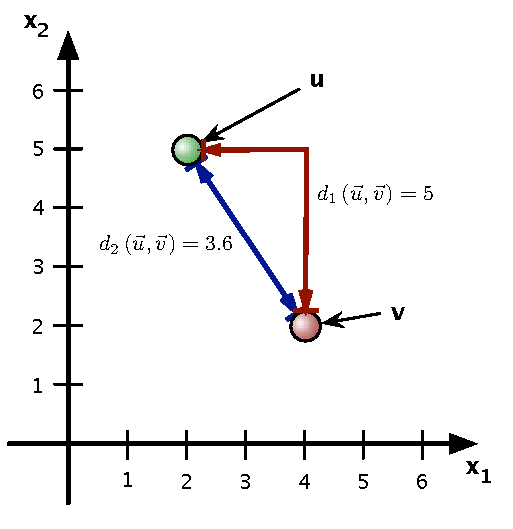
\includegraphics[width=45mm]{img/7_distance_examples}
    \end{column}
  \end{columns}
  \gap[.5]
  \only<beamer:2| handout:0>{%
    \[ \dist[2]{\vu}{\vv} \coloneq \sqrt{(u_1 - v_1)^2 + \dots + (u_n - v_n)^2} \] }
  \only<beamer:3| handout:0>{%
    \[ \dist[1]{\vu}{\vv} \coloneq \abs{u_1 - v_1} + \dots + \abs{u_n - v_n} \] }
  \only<beamer:4-| handout:1>{%
    \[ \dist[p]{\vu}{\vv} \coloneq \bigl(
    \abs{u_1 - v_1}^p + \dots + \abs{u_n - v_n}^p
    \bigr)^{1/p} \] }
  \only<beamer:5-| handout:1>{%
    \[ \dist[\infty]{\vu}{\vv} = \max \bigset{\abs{u_1 - v_1}, \ldots, \abs{u_n - v_n}} \] }
\end{frame}

\begin{frame}
  \frametitle{Geometric distance = metric}
  %% \framesubtitle{}

  \begin{columns}[T]
    \begin{column}{60mm}
      \begin{itemize}
      \item \hh{Distance} between vectors $\vu, \vv \in \setR^n$ \so
        (dis)similarity
        \begin{itemize}
        \item $\vu = (u_1, \ldots, u_n)$
        \item $\vv = (v_1, \ldots, v_n)$
        \end{itemize}
      \item \h{Euclidean} distance $\dist[2]{\vu}{\vv}$
      \item ``City block'' \h{Manhattan} distance $\dist[1]{\vu}{\vv}$
      \item Extension of $p$-distance  $\dist[p]{\vu}{\vv}$ (for $0\leq p\leq 1$)
      \end{itemize}
    \end{column}
    \begin{column}{45mm}
      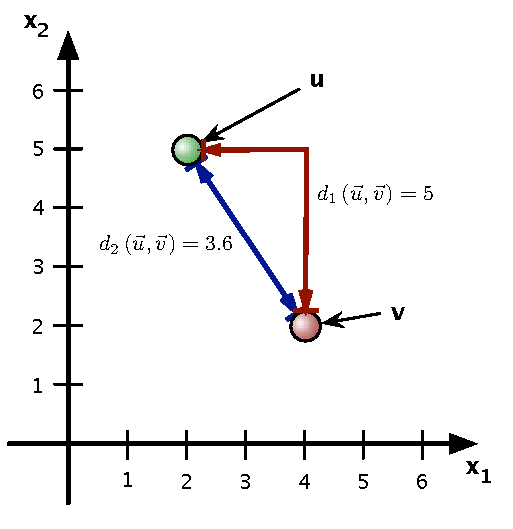
\includegraphics[width=45mm]{img/7_distance_examples}
    \end{column}
  \end{columns}
  \gap[1.5]
  \[ \dist[p]{\vu}{\vv} \coloneq \abs{u_1 - v_1}^p + \dots + \abs{u_n - v_n}^p \]
  \[ \dist[0]{\vu}{\vv} = \# \bigsetdef{i}{u_i \neq v_i} \]
\end{frame}

\begin{frame}
  \frametitle{Distance and vector length = norm}
  %% \framesubtitle{}

  \ungap[1]
  \begin{columns}[T]
    \begin{column}{50mm}
      \begin{itemize}
      \item<1-> Intuitively, distance $\dist{\vu}{\vv}$ should correspond to
        length $\norm{\vu-\vv}$ of displacement vector $\vu - \vv$
        \begin{itemize}
        \item $\dist{\vu}{\vv}$ is a \h{metric}
        \item $\norm{\vu-\vv}$ is a \h{norm}
        \item $\norm{\vu} = \bigdist{\vu}{\vnull}$
        \end{itemize}
      \item<2-> Any norm-induced metric is \h{translation-invariant}%
        \gap
      \item<3-> $\dist[p]{\vu}{\vv} = \norm[p]{\vu-\vv}$
      \end{itemize}
    \end{column}
    \begin{column}{50mm}
      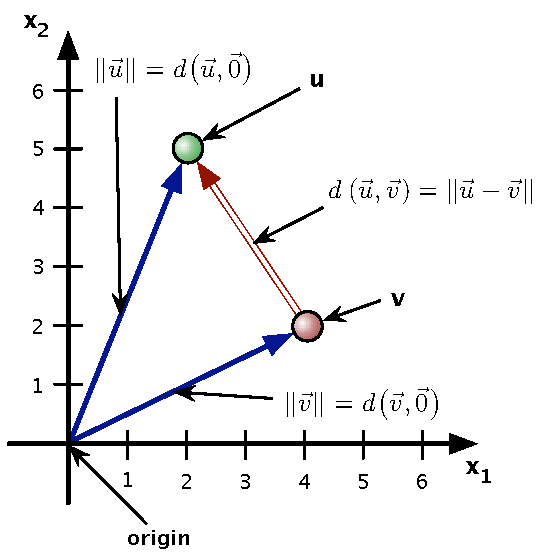
\includegraphics[width=50mm]{img/7_distance_norm}
    \end{column}
  \end{columns}

  \gap
  \begin{itemize}
  \item<3-> \h{Minkowski $p$-norm} for $p\in [1,\infty]$ (not $p < 1$):
    \[
    \norm[p]{\vu} \coloneq \bigl(\abs{u_1}^p + \dots + \abs{u_n}^p\bigr)^{1/p}
    \]
  \end{itemize}
\end{frame}

\begin{frame}
  \frametitle{Angular distance = cosine similarity}
  % \framesubtitle{}

  \ungap[1]
  \begin{columns}[c]
    \begin{column}{5cm}
      \begin{itemize}
        \item Angle $\alpha$ between vectors $\vu,\vv\in \setR^n$ is given by
          \begin{align*}
            \cos \alpha &= 
            \frac{\sum_{i=1}^n u_i\cdot v_i}{
              \sqrt{\sum_i u_i^2}\cdot \sqrt{\sum_i v_i^2}}
            \\
            &= \frac{\vu^T \vv}{\norm[2]{\vu}\cdot \norm[2]{\vv}}
        \end{align*}
      \item<2-> Corresponding metric: \h{angular distance} $\alpha$
      \end{itemize}
    \end{column}
    \begin{column}{5cm}
      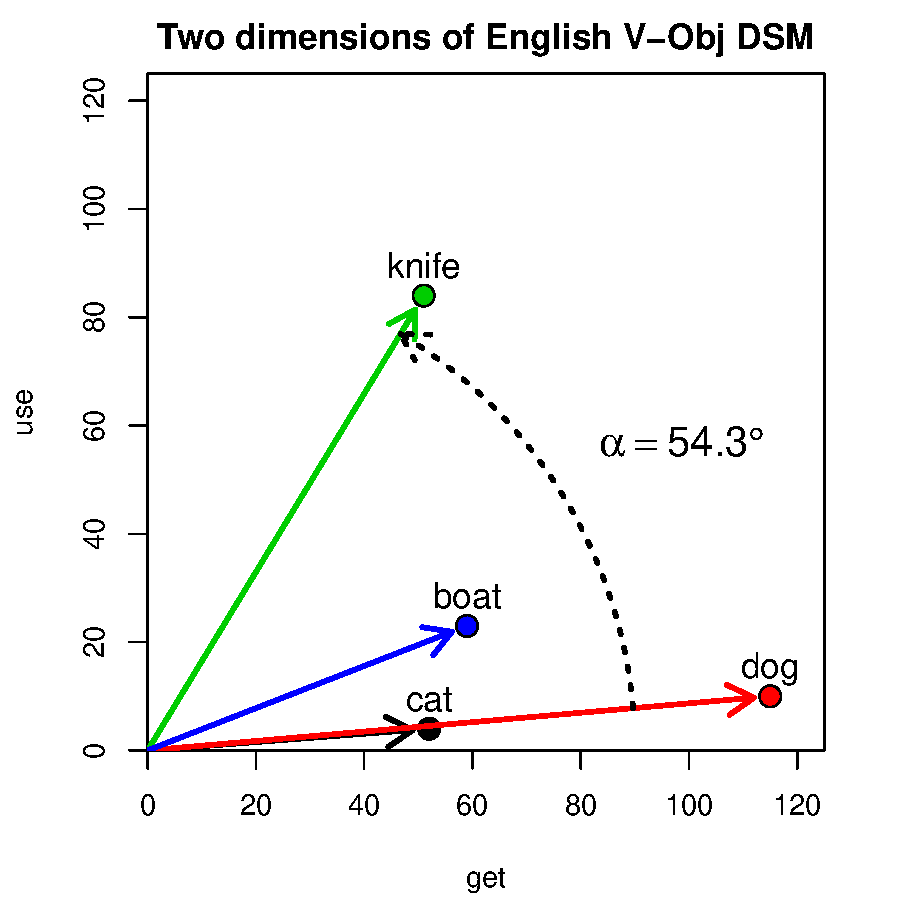
\includegraphics[width=5cm]{img/angular_distance_hieroglyph}
    \end{column}
  \end{columns}

  \gap
  \begin{itemize}
  \item<2-> $\alpha$ is a metric on direction vectors (regardless of length)
  \item<3-> \hh{Cosine} measure of similarity: $\cos \alpha$
    \begin{itemize}
    \item $\cos \alpha = 1$ \so collinear
    \item $\cos \alpha = 0$ \so \h{orthogonal}
    \end{itemize}
  \end{itemize}
\end{frame}

\todoslide[TODO: angles \& orthogonality]{
  dot product, angle, cosine similarity;
  relation to Euclidean metric; orthogonality}

\begin{frame}[fragile]
  \frametitle{Computing distances}

Compute distances between all pairs of texts:
\begin{Rcode}
> round(dist(M), 2)  \REM{returns a triangular `dist' object}
> round(dist(M, method="manhattan"), 2) \REM{Manhattan metric}
\end{Rcode}

\gap[1]\pause
Use \texttt{wordspace} function for additional metrics:
\begin{Rcode}
> dist.matrix(M, method="mink", p=0.5)  \REM{full matrix}
> dist.matrix(M, method="mink", p=0.5, as.dist=TRUE)
\end{Rcode}

\gap[1]\pause
Standardize features for equal contribution to Euclidean metric:
\begin{Rcode}
> Z <- scale(M)     \REM{matrix of z-scores}
> round(dist(Z), 2) \REM{default: Euclidean metric}
\end{Rcode}
\end{frame}

%%%%%%%%%%%%%%%%%%%%%%%%%%%%%%%%%%%%%%%%%%
\subsection{Orthogonal projection}

\begin{frame}
  \frametitle{Linear subspace \& basis}
  
  \begin{itemize}
  \item A linear \h{subspace} $B\subseteq \setR^n$ of rank $r\leq n$ is spanned by a set of $r$ linearly independent basis vectors
    \[
    B = \set{\vb_1, \ldots, \vb_r}
    \]
  \end{itemize}

  \begin{columns}[T]
    \begin{column}{55mm}
      \begin{itemize}
      \item<2-> Every point $\vu$ in the subspace is a unique linear combination of the basis vectors
        \[
          \vu = x_1 \vb_1 + \ldots + x_r \vb_r
        \]
      \item<2-> Coordinate vector $\vx\in \setR^r$ with respect to the basis
      \end{itemize}
    \end{column}
    \begin{column}{45mm}
      \hspace*{-5mm}%
      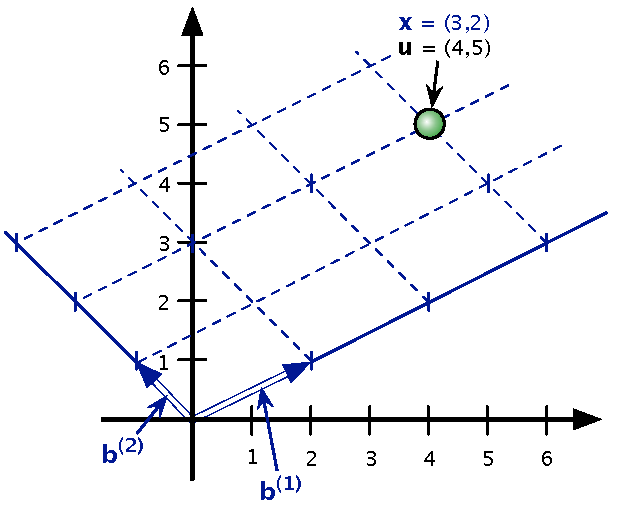
\includegraphics[width=55mm]{img/7_basis_grid}  
    \end{column}
  \end{columns}
\end{frame}

\begin{frame}
  \frametitle{Linear subspace \& basis}
  
  \begin{itemize}
  \item Basis matrix $\mathbf{V} \in \setR^{n\times r}$ with column vectors $\vb_i$:
    \[
    \vu = x_1 \vb_1 + \ldots + x_r \vb_r = \mathbf{V} \vx
    \]
  \end{itemize}

  \[
  \begin{array}{ccccc}
    \begin{bmatrix}
      x_1 b_{11} + \ldots + x_r b_{1r} \\
      x_1 b_{21} + \ldots + x_r b_{2r} \\
      \vdots\\
      x_1 b_{n1} + \ldots + x_r b_{nr}
    \end{bmatrix}
    & = &
    \begin{bmatrix}
      b_{11} & \cdots & b_{1r} \\
      b_{21} & \cdots & b_{2r} \\
      \vdots & & \vdots \\
      b_{n1} & \cdots & b_{nr}
    \end{bmatrix}
    & \cdot &
    \begin{bmatrix}
      x_1 \\
      \vdots \\
      x_r
    \end{bmatrix} \\
    \\
    \mathbf{u} & = & \mathbf{V} & \cdot & \mathbf{x} \\
    (n\times 1) & & (n\times \primary{r}) & & (\primary{r}\times 1)
  \end{array}
  \]

\end{frame}

\begin{frame}
  \frametitle{An aside: Matrix multiplication}
  %% \framesubtitle{}

  \ungap
  \[
  \begin{array}{ccccc}
    \begin{bmatrix}
      & \only<beamer:2| handout:0>{a_{ij}} & \only<beamer:1| handout:0>{a_{ij}} & \\
      \only<beamer:3| handout:1>{a_{ij}} & & & \\
      & & &
    \end{bmatrix}
    & = &
    \begin{bmatrix}
      \only<beamer:1-2| handout:0>{b_{i1}} & \only<beamer:1-2| handout:0>{\cdots} & \only<beamer:1-2| handout:0>{b_{in}} \\
      \only<beamer:3| handout:1>{b_{i1}} & \only<beamer:3| handout:1>{\cdots} & \only<beamer:3| handout:1>{b_{in}} \\
      & &  
    \end{bmatrix}
    & \cdot &
    \begin{bmatrix}
     \only<beamer:3| handout:1>{c_{1j}}   & \only<beamer:2| handout:0>{c_{1j}} & \only<beamer:1| handout:0>{c_{1j}} &\\
     \only<beamer:3| handout:1>{\vdots}   & \only<beamer:2| handout:0>{\vdots} & \only<beamer:1| handout:0>{\vdots} & \\
     \only<beamer:3| handout:1>{\vdots}   & \only<beamer:2| handout:0>{\vdots} & \only<beamer:1| handout:0>{\vdots} & \\
     \only<beamer:3| handout:1>{c_{nj}}   & \only<beamer:2| handout:0>{c_{nj}} & \only<beamer:1| handout:0>{c_{nj}} & 
    \end{bmatrix} \\
    \\
    \mathbf{A} & = & \mathbf{B} & \cdot & \mathbf{C} \\
    (k\times m) & & (k\times \primary{n}) & & (\primary{n}\times m)
  \end{array}
  \]
  \begin{itemize}
  \item $\mathbf{B}$ and $\mathbf{C}$ must be \h{conformable} (in dimension \primary{$n$})
  \item Element $a_{ij}$ is the inner product of the $i$-th row of $\mathbf{B}$ and the $j$-th column of $\mathbf{C}$
    \[
    a_{ij} = b_{i\primary{1}} c_{\primary{1}j} + \ldots + b_{i\primary{n}} c_{\primary{n}j} = \sum_{t=1}^n b_{i\primary{t}} c_{\primary{t}j}
    \]
  \end{itemize}
\end{frame}

\begin{frame}
  \frametitle{Orthonormal basis}

  \begin{itemize}
  \item Particularly convenient with orthonormal basis:
    \begin{align*}
      \norm[2]{\vb_i} &= 1 \\
      \vb_i^T \vb_j &= 0 && \text{for } i\neq j
    \end{align*}
  \item Corresponding basis matrix $\mathbf{V}$ is (column)-\hh{orthogonal}
    \[
      \mathbf{V}^T \mathbf{V} = \mathbf{I}_r
    \]
    and defines a \primary{Cartesian coordinate system} in the subspace
    \begin{itemize}
    \item[]
    \end{itemize}
  \item<2->[\hand] From now on always assume orthonormal basis
  \end{itemize}
\end{frame}

\begin{frame}
  \frametitle{The mathematics of projections}
  %% \framesubtitle{}

  \begin{columns}[c]
    \begin{column}{50mm}
      \begin{itemize}
      \item 1-d subspace spanned by basis vector
        $\norm[2]{\vb} = 1$
      \item For any point $\vu$, we have
        \[
          \cos \varphi
          = \frac{\vb^T \vu}{\norm[2]{\vb}\cdot \norm[2]{\vu}}
          = \frac{\vb^T \vu}{\norm[2]{\vu}}          
        \]
      \item<2-> Trigonometry: coordinate of point on the line is
        $x = \norm[2]{\vu}\cdot \cos\varphi = \vb^T \vu$
      \end{itemize}
    \end{column}
    \begin{column}{50mm}
      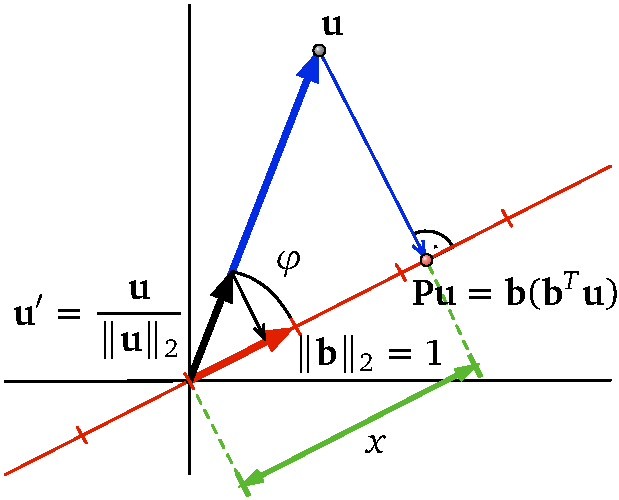
\includegraphics[width=50mm]{img/7_cosine_projection}
    \end{column}
  \end{columns}
  
  \begin{itemize}
  \item<3-> The projected point in original space is then given by
    \[
      \vb\cdot x = \vb (\vb^T \vu) = (\vb \vb^T) \vu = \mathbf{P} \vu
    \]
    where $\mathbf{P}$ is a \h{projection matrix} of rank 1
  \end{itemize}
\end{frame}

\begin{frame}
  \frametitle{The mathematics of projections}
  %% \framesubtitle{}

  \begin{itemize}
  \item For an orthogonal basis matrix $\mathbf{V}$ with columns
    $\vb_1, \ldots, \vb_r$, the projection into the rank-$r$ subspace $B$ is
    given by
    \[
      \mathbf{P}\vu = \left(\sum_{i=1}^r \vb_i \vb_i^T\right) \vu
      = \mathbf{V} \mathbf{V}^T \vu
    \]
    and its subspace coordinates are $\vx = \mathbf{V}^T \mathbf{u}$
  \item<2-> Projection can be seen as decomposition into the projected vector
    and its orthogonal complement
    \[
      \vu = \mathbf{P} \vu + (\vu - \mathbf{P} \vu)
      = \mathbf{P} \vu + (\mathbf{I} - \mathbf{P}) \vu
      = \mathbf{P} \vu + \mathbf{Q} \vu
    \]
  \item<3-> Because of orthogonality, this also applies to the squared
    Euclidean norm (according to the Pythagorean theorem)
    \[
      \norm{\vu}^2 = \norm{\mathbf{P} \vu}^2 + \norm{\mathbf{Q} \vu}^2
    \]
  \end{itemize}
\end{frame}

\begin{frame}
  \frametitle{Optimal projections and subspaces}
  %% \framesubtitle{}

  \begin{itemize}
  \item Orthogonal decomposition of squared distances btw.\ vectors
    \[
      \norm{\vu - \vv}^2 = \norm{\mathbf{P} \vu - \mathbf{P} \vv}^2 + \norm{\mathbf{Q} \vu - \mathbf{Q} \vv}^2
    \]
  \end{itemize}

  \begin{columns}[c]
    \begin{column}{60mm}
      \begin{itemize}
      \item<2-> Define projection \hh{loss} as difference btw.\ squared distances
        \begin{align*}
          & \bigabs{\,\norm{\mathbf{P}(\vu - \vv)}^2 - \norm{\vu - \vv}^2\,} \\
          =\;& \norm{\vu - \vv}^2 - \norm{\mathbf{P}(\vu - \vv)}^2 \\
          =\;& \norm{\mathbf{Q}(\vu - \vv)}^2
        \end{align*}
      \item<3-> Projection quality measure:
        \[
          R^2 = \frac{\norm{\mathbf{P}(\vu - \vv)}^2}{\norm{\vu - \vv}^2}
        \]
      \end{itemize}
    \end{column}
    \begin{column}{40mm}
      \hspace*{-5mm}%
      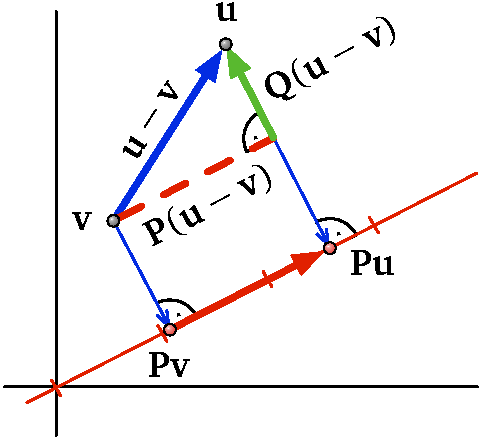
\includegraphics[width=45mm]{img/7_projection_loss}      
    \end{column}
  \end{columns}
\end{frame}

%%%%%%%%%%%%%%%%%%%%%%%%%%%%%%%%%%%%%%%%%%%%%%%%%%%%%%%%%%%%%%%%%%%%%%
\section{Exploratory techniques}

%%%%%%%%%%%%%%%%%%%%%%%%%%%%%%%%%%%%%%%%%%
\subsection{Clustering}

\todoslide{hierarchical and flat clustering; examples}

\todoslide{seriation \& over/underuse; examples}

%%%%%%%%%%%%%%%%%%%%%%%%%%%%%%%%%%%%%%%%%%
\subsection{Visualisation}

\todoslide{GMA visualisation functions + 3D}

\todoslide{embeddings: MDS, t-SNE, etc.}


%%%%%%%%%%%%%%%%%%%%%%%%%%%%%%%%%%%%%%%%%%%%%%%%%%%%%%%%%%%%%%%%%%%%%%
\section{Geometric multivariate analysis (GMA)}

\todoslide[TODO]{Introduce GMA functions for subspaces}

%%%%%%%%%%%%%%%%%%%%%%%%%%%%%%%%%%%%%%%%%% 
\subsection{PCA and factor analysis}

\todoslide[TODO: PCA and SVD]{
  find best projection into single dimension (illustration from wordspace);
  mathematics: covariance matrix, optimal basis vector $\mathbf{b}$;
  eigenvalue decomposition as generalisation?;
  SVD, properties $\to$ optimal projection}

\todoslide[TODO: factor analysis]{
  similar to PCA, just different objective;
  here focus on geometric approach with PCA}

\todoslide{PCA in R/GMA; examples}

%%%%%%%%%%%%%%%%%%%%%%%%%%%%%%%%%%%%%%%%%%
\subsection{Linear discriminant analysis (LDA)}

\todoslide[TODO: LDA]{
  linear discriminant analysis to focus on specific aspects of fine-grained patterns;
  projection as perspective on data; main shape (PCA) + salient structure (LDA);
  discussion of minimal supervision}

\todoslide{LDA in R/GMA; examples and interpretation}

%%%%%%%%%%%%%%%%%%%%%%%%%%%%%%%%%%%%%%%%%%
\subsection{Interpreting dimensions}

\todoslide{interpretation of latent dimensions; weights, boxplots, etc.}

%%%%%%%%%%%%%%%%%%%%%%%%%%%%%%%%%%%%%%%%%%
\subsection{Validation }

\begin{frame}
  \frametitle{Comparing subspaces}

  We want to compare two subspaces $A$ and $B$ of the same dimensionality $r \leq n$, with
  orthonormal basis vectors
  \begin{itemize}
  \item $\va_1, \ldots, \va_r$ = \secondary{column} vectors of basis matrix $\mathbf{A}$
  \item $\vb_1, \ldots, \vb_r$ = \secondary{column} vectors of basis matrix $\mathbf{B}$
  \end{itemize}

  \[
    \vz = \mathbf{B} \vx =
    \begin{bmatrix}
      \vdots & & \vdots \\
      \vb_1 & \cdots & \vb_r \\
      \vdots & & \vdots
    \end{bmatrix}
    \cdot
    \begin{bmatrix}
      x_1 \\
      \vdots \\
      x_r
    \end{bmatrix}
  \]
  
  \begin{itemize}
  \item[\hand] $\vx\in \setR^r$ are the subspace coordinates of a vector $\vz\in B$
  \end{itemize}
\end{frame}

\todoslide[TODO: illustration]{
  diagram of two oblique 2-dim subspaces overlapping in one dimension that's not aligned with their basis vectors;
  work out something where both the original basis vectors and the intersection are relatively simple numbers}

\begin{frame}
  \frametitle{Projection between subspaces}

  \begin{itemize}
  \item The projection of $\vz$ into subspace $A$ is
    \[
      \mathbf{P} \vz = \mathbf{A} \mathbf{A}^T \vz = \mathbf{A} \vy
    \]
    with $\vy\in \setR^r$ = subspace coordinates of the projection in $A$
  \item Hence the projection from subspace coordinates in $B$ to subspace coordinates in $A$ is given by
    \[
      \vy = \mathbf{A}^T \vz = (\mathbf{A}^T \mathbf{B}) \vx
    \]
  \item \TODO[example + illustration]
  \end{itemize}
\end{frame}

\begin{frame}
  \frametitle{Goals}

  \h{Determine overlap}
  \begin{itemize}
  \item<2-> Identify dimensions that $A$ and $B$ have in common
  \item<2-> Overlap = number of shared dimensions ($\neq$ basis vectors)
  \end{itemize}

  \h{Measure similarity of subspaces}
  \begin{itemize}
  \item<3-> Average $R^2$ of projection from $B$ to $A$ (\hand{} symmetric?)
    \begin{itemize}
    \item either for random vectors in $B$ (standard multivariate normal)
    \item or for a specific data set $M$
    \end{itemize}
  \item<4-> Overlap + cosine similarity
    \begin{itemize}
    \item number of shared dimensions plus
    \item cosine btw.\ each non-shared dimension in $B$ and subspace $A$
    \item prerequisite: find matching basis vectors in $B$ and $A$
    \end{itemize}
  \item<5-> ``Volume'' of projection image
    \begin{itemize}
    \item determinant of $\set{\mathbf{P}\vb_1, \ldots, \mathbf{P}\vb_r}$
    \item not useful: single orthogonal dimension \so{} determinant = 0
    \end{itemize}
  \end{itemize}
\end{frame}

\begin{frame}
  \frametitle{Matching basis vectors between subspaces}

  \begin{itemize}
  \item Rotate orthornomal basis vectors in both subspaces so that the new bases $\vc_1,\ldots, \vc_r$ of $A$ and $\vd_1, \ldots, \vd_r$ of $B$ are matched under projection, i.e.
    \begin{align*}
      \vc_i &= \vd_i = \mathbf{P} \vd_i &&\text{for shared dimensions}\\
      \sigma_j \vc_j &= \mathbf{P} \vd_j &&\text{otherwise}
    \end{align*}
    (in short: $\sigma_i \vc_i = \mathbf{P} \vd_i$ with $\sigma_i = 1$ for shared dimensions)
  \item<2-> Using subspace coordinates $\vc_i = \mathbf{A} \vu_i$ and $\vd_i = \mathbf{B} \vv_i$, we have
    \[
      \sigma_i \vu_i
      = \mathbf{A}^T \underbrace{\mathbf{A} \mathbf{A}^T}_{\mathbf{P}} \mathbf{B} \vv_i
      = \underbrace{\mathbf{A}^T \mathbf{A}}_{\mathbf{I}_r} \mathbf{A}^T \mathbf{B} \vv_i
      = (\mathbf{A}^T \mathbf{B}) \vv_i
    \]
  \item<2-> Therefore, $\vu_i$ and $\vv_i$ are left and right singular vectors of $\mathbf{A}^T \mathbf{B}$
  \end{itemize}
\end{frame}

\begin{frame}
  \frametitle{Matching basis vectors between subspaces}

  \begin{itemize}
  \item Singular value decomposition (SVD) of $\mathbf{A}^T \mathbf{B}$:
    \[
      \mathbf{A}^T \mathbf{B} = \mathbf{U} \Msigma \mathbf{V}^T
      = \sum_{i=1}^r \sigma_i \vu_i \vv_i^T
    \]
  \item[\hand] It is easy to see that $(\mathbf{A}^T \mathbf{B}) \vv_j = \sigma_j \vu_j$ as required
  \item<2-> Matching basis vectors for $A$ and $B$ are thus given by
    \[
      \vc_i = \mathbf{A} \vu_i \;\so{}\; \mathbf{C} = \mathbf{AU} \qquad
      \vd_i = \mathbf{B} \vv_i \;\so{}\; \mathbf{D} = \mathbf{BV}
    \]
    (both are orthonormal because $\mathbf{U}$ and $\mathbf{V}$ are orthogonal)
  \item<3-> And projection $\mathbf{P} \vz$ in the new coordinates reduces to
    \[
      \vy' = \mathbf{C}^T \mathbf{P} \vz = \mathbf{C}^T \mathbf{D} \vx'
      = \mathbf{U}^T \underbrace{\mathbf{A}^T\mathbf{B}}_{\mathbf{U}\Msigma\mathbf{V}^T} \mathbf{V} \vx'
      = \Msigma \vx'
    \]
  \end{itemize}
\end{frame}

\begin{frame}
  \frametitle{Shared dimensions and subspace similarity}

  \begin{itemize}
  \item Every shared dimension has singular value $\sigma_i = 1$, i.e.
    \[
      \#\text{shared}(A, B) = \abs{\set{\sigma_i = 1}}
    \]
  \item For other dimensions, $\sigma_j$ is the cosine similarity
    \[
      \vc_j^T \vd_j = (\mathbf{C}^T \mathbf{D})_{jj} = \Msigma_{jj} = \sigma_j
    \]
  \item Similarity \h{measure of shared dimensionality} is given by
    \[
      \text{Sim}_1(A, B) = \sum_{i=1}^r \sigma_i
    \]
    \begin{itemize}
    \item[\hand] Sim$_1$ ranges from $0$ (fully orthogonal) to $r$ (identical)
    \item[\hand] Sim$_1$ is symmetric (because of symmetry of SVD)
    \end{itemize}
  \end{itemize}
\end{frame}

\begin{frame}
  \frametitle{Similarity as preserved variance}

  \begin{itemize}
  \item For random vectors $\vx \sim N_r(\vnull, \mathbf{I})$ in $B$ (subspace coord)
    \begin{itemize}
    \item rotation to $\mathbf{C}$ and $\mathbf{D}$ doesn't affect distribution:
      $\vx' \sim N_r(\vnull, \mathbf{I})$
    \item projection $\vy' = \mathbf{C}^T \mathbf{D} \vx' = \Msigma \vx' \sim N_r(\vnull, \Msigma^2)$
      \[
        \frac{ \Exp{\norm{\vy'}^2} }{ \Exp{\norm{\vx'}^2} }
        = \frac{ \sum_{i=1}^r \sigma_i^2 }{ r }
      \]
    \end{itemize}
  \item Expected \h{proportion of preserved variance} is thus
    \[
      \text{Sim}_2(A, B) = \frac1r \sum_{i=1}^r \sigma_i^2
    \]
    \begin{itemize}
    \item[\hand] Sim$_2$ ranges from $0$ (fully orthogonal) to $1$ (identical)
    \end{itemize}
  \item $\text{Sim}_2(B, A) = \text{Sim}_2(A, B)$ because the reverse projection  from $A$ to $B$ is
    $\mathbf{B}^T\mathbf{A} = (\mathbf{A}^T\mathbf{B})^T = \mathbf{V}\Msigma\mathbf{U}^T$ with same $\Msigma$
  \end{itemize}  
\end{frame}


\todoslide[TODO: Bootstrapping \& cross-validation]{
  bootstrapping \& cross-validation to estimate overtraining / uncertainty;
  measure ``wobble'' of dimensions; cross-validate coordinates;
  distribution of feature weights}

% %%%%%%%%%%%%%%%%%%%%%%%%%%%%%%%%%%%%%%%%%%%%%%%%%%%%%%%%%%%%%%%%%%%%%%
% \section{}

% %%%%%%%%%%%%%%%%%%%%%%%%%%%%%%%%%%%%%%%%%%
% \subsection{}

% \begin{frame}
%   \frametitle{}
%   % \framesubtitle{}

% \end{frame}

% \begin{frame}[fragile]
%   \frametitle{}
%   %% \framesubtitle{}

%   % \ungap[1]
%   \begin{alltt}
%   \end{alltt}
% \end{frame}

%%%%%%%%%%%%%%%%%%%%%%%%%%%%%%%%%%%%%%%%%%%%%%%%%%%%%%%%%%%%%%%%%%%%%%
%% References (if any)

\frame[allowframebreaks]{
  \frametitle{References}
  \bibliographystyle{natbib-stefan}
  \begin{scriptsize}
    \bibliography{sigil}
  \end{scriptsize}
}

\end{document}
